\chapter{Implementation}



\section{ER/Studio}

\subsection{File Reverse-Engineering Tool}
\label{subsec:dm1_tool}

We need to decrypt relations between tables in ER/Studio .DM1 files in order to be able to deconstruct objects stored in the files. 
We described the file format together with the need for help in \autoref{subsec:dm1_format}.
The task is to find out what links are leading between tables in the format. The links are done via primary and foreign keys.

Input is an arbitrary .DM1 file and output must describe the logical layout. 
We proposed the parallel with relational databases which can be represented understandably by a relational diagram, we will try to visualize the result showing organization of the format by such diagram. 
For creation of relational diagram a modeling tools are used. 
If we are able to generate a SQL code definition of the file format enriched with definition of primary and foreign keys, modeling tools can transform such code into a visual representation of database structure that is creates.

Modeling tools commonly have the ability of reverse engineer a database, however they do it based on metadata from a deployed database where keys are defined. 
If we just described tables in .DM1 file format by SQL creates, there is no tool that could effectively infer relations. That is why we need this reverse-engineering tool.
As the development of such tool is not the focal point of the work, this will be not an out-box general solution for deducing keys for relational databases, but will provide a basic overview of .DM1 file organization. Also it is not a complete solution but is primarily aimed on the objects and properties we picked by analysis. \TODO{reference}

The decision what programming language should be used for the discussed fell to Java as the final Metadata Extractor was going to be written in the language and there are units we want to reuse in this tool as well as in further parts. Although there may be scripting languages that would make some operations, like joins on tables easier.
For example in order to go through the file format a parser is needed. Instead of writing it multiple times we will write it once in Java and use here just like in Metadata Extractor itself. \\

The idea is to look at the tables from two views.

The first one is to take into account only metadata which is represented by the class DependencyCreator. It treats column that looks like keys (eg. those which name ends with "ID", the policy is determined by isOnBlacklist method) as the same across all tables. 
The main method here is createDependencies which pairs potential key columns and tables in what they are used.
Then there is the class RelationFinderByTableDefinitions that allows querying over the structure found by DependecyCreator showing what tables are possibly related through a series of joins.
Among other there is the general method getDependenciesWithPaths is showing a sequence of joins needed to do in order to put put together records from table a with those from table b.

The second view takes into account the data stored in tables as well. 
When analyzing what are relations between columns, we see a table as a collection of columns, where a column has a set of values. This way we can examine if columns with same names have similar contents.
In contrast when getting records from a table we see a collection of rows.
The RelationFinderByTableContents class is used for the further search for key columns.

It filters tables that without content, thus irrelevant.
Has method for determining if a column can be considered a primary key of a table, that is when it contains only distinct ids.
Method for finding out if a column can be foreign key corresponding to primary key column, thus the first one contains subset of values for the other.
In .DM1 file format there is a table Identity Value that explicitly pairs tables with their primary keys. 
The class also inspects if the primary keys are defined in strict order or if there is some pattern key definitions follow.

The classes above are used for being able to look from multiple perspectives and to comprehend the format.
To put it all together and finally generate the desired output in form of a SQL definition of .DM1 tables in SQL with keys out of the analysis the class TablesToSQLConverter is used.
The main method is writeMySQLSource that at first defines create table procedure for each table from ER/Studio source. 
Then the phase of creating key constraints takes place. It operates on candidate columns that satisfy policies in DepedencyCreator to be key column and are present in at least one table so at least one join can be made using them.
There is also space for defining manually the knowledge we gained by inspecting the format using RelationFinder* classes by inserting pairs table-primary keys.
So primary keys are defined from user-defined information, the information stored in Identity Value table and are inferred based on policies taking into account name of a column and name of the table it belongs to.
If a column is set as a primary key in one table for each of the remaining ones that contain it, it is marked as a foreign identifier.
In case there are columns that are candidates for being keys but no source table was assigned to them in previous steps one of the tables is chosen as the source, that may cause inaccuracies in the final result but the main message should not get lost.

\subsection{Parser}
\label{subsec:dm1_parser}

Existing CSV parsers are made to process a single CSV structure per file. There is no unified definition for the comma-separated-value files, but usually they do not allow naming CSV tables as present in .DM1 files.
What is important to say about CSV record is that each entry is on a located on a separate line, fields in an entry are separated by a comma, the last record is followed by line break. A field may contain a comma or line break but must be enclosed by quotes. 
If a double quote appears in a field, it must be in the enclosed section and the quote itself must be doubled. \TODO{https://tools.ietf.org/html/rfc4180} 

We know the structure we need to parse contains tables consisting of a name on a single line, definition of columns and entries. Two tables are separated by a single empty line.

Putting it all together it seems to be easier to come with an own parser for .DM1 files that processes the files into a set of tables identified by their names. 

\TODO{parser for RE vs for Connector}
To represent a single table we have the class \classname{CSVTable} which contains its name, definition of columns, in other words names for each of its property\TODO{name of the class}, and finally records themselves - instances of \classname{CSVColumn} which are contents of the table.

Getting a name of a table is an easy job as its just a single textual line. To resolve a record is a slightly more challenging task. We design an automaton that accepts well formed records of our CSV table.

\TODO{in I and F states a field is added to record}
\TODO{alphabet}
\TODO{NFA}

\begin{center}
	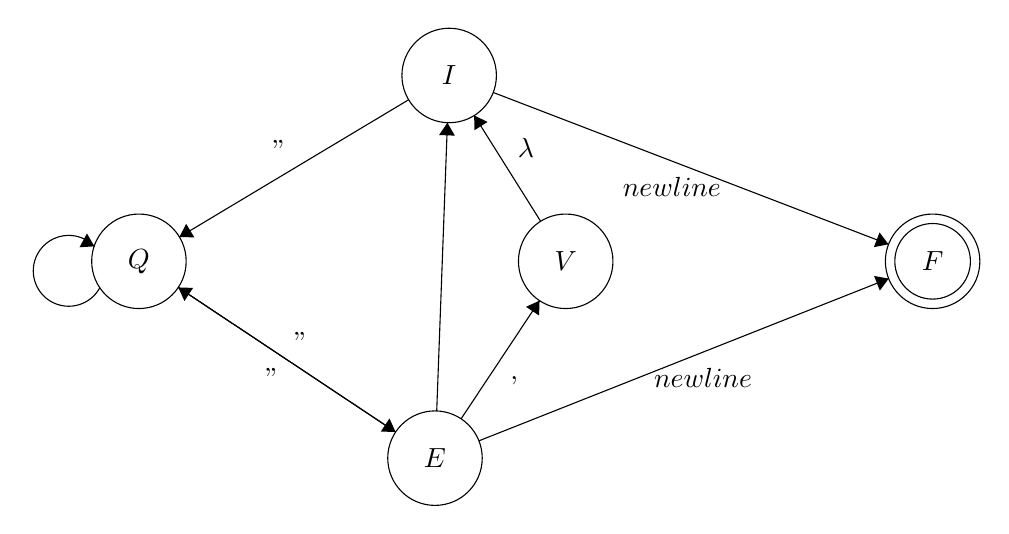
\begin{tikzpicture}[scale=0.2]
	\tikzstyle{every node}+=[inner sep=0pt]
	\draw [black] (40.8,-21.4) circle (3);
	\draw (40.8,-21.4) node {$I$};
	\draw [black] (71.5,-33.2) circle (3);
	\draw (71.5,-33.2) node {$F$};
	\draw [black] (71.5,-33.2) circle (2.4);
	\draw [black] (21.1,-33.2) circle (3);
	\draw (21.1,-33.2) node {$Q$};
	\draw [black] (48.2,-33.2) circle (3);
	\draw (48.2,-33.2) node {$V$};
	\draw [black] (39.9,-45.7) circle (3);
	\draw (39.9,-45.7) node {$E$};
	\draw [black] (43.6,-22.48) -- (68.7,-32.12);
	\fill [black] (68.7,-32.12) -- (68.13,-31.37) -- (67.77,-32.3);
	\draw (54.94,-27.83) node [below] {$newline$};
	\draw [black] (38.23,-22.94) -- (23.67,-31.66);
	\fill [black] (23.67,-31.66) -- (24.62,-31.68) -- (24.1,-30.82);
	\draw (30.04,-26.8) node [above] {$"$};
	\draw [black] (18.622,-34.87) arc (-28.28273:-316.28273:2.25);
	\fill [black] (18.27,-32.25) -- (17.8,-31.43) -- (17.33,-32.31);
	\draw [black] (23.6,-34.86) -- (37.4,-44.04);
	\fill [black] (37.4,-44.04) -- (37.01,-43.18) -- (36.46,-44.01);
	\draw (29.59,-39.95) node [below] {$"$};
	\draw [black] (42.69,-44.6) -- (68.71,-34.3);
	\fill [black] (68.71,-34.3) -- (67.78,-34.13) -- (68.15,-35.06);
	\draw (56.92,-39.97) node [below] {$newline$};
	\draw [black] (41.56,-43.2) -- (46.54,-35.7);
	\fill [black] (46.54,-35.7) -- (45.68,-36.09) -- (46.51,-36.64);
	\draw (44.66,-40.78) node [right] {$,$};
	\draw [black] (37.4,-44.04) -- (23.6,-34.86);
	\fill [black] (23.6,-34.86) -- (23.99,-35.72) -- (24.54,-34.89);
	\draw (31.41,-38.95) node [above] {$"$};
	\draw [black] (40.01,-42.7) -- (40.69,-24.4);
	\fill [black] (40.69,-24.4) -- (40.16,-25.18) -- (41.16,-25.22);
	\draw [black] (46.61,-30.66) -- (42.39,-23.94);
	\fill [black] (42.39,-23.94) -- (42.4,-24.88) -- (43.24,-24.35);
	\draw (45.13,-26.01) node [right] {$\lambda$};
	\end{tikzpicture}
\end{center}

\TODO{if malformed}

The parser's interface is a single method \methodname{readFile} taking a file to process and returning pairs of table name and an instance of \classname{CSVTable}.

\subsection{Model}

The purpose of the model unit is to provide an access for reading to both a raw structure of a processed source file and a fully loaded hierarchy of objects we reconstructed from the file.

The crucial objects and the important properties of theirs result from the analysis of ER/Studio data models \TODO{reference to the section}. Those are the ones the model is required to capture.

The perspective of a raw file structure loaded to memory is represented by an interface \classname{ErStudioFile} where either all tables from file can be retrieved via \methodname{getAllCsvTables} or a single table by its name using the \methodname{getCsvTable} method.

An ER/Studio solution - a set containing one logical data model and arbitrary number of physical models implements \classname{ErStudioSolution} interface. All the objects contained in the data models stored in such solution can be retrieved using the interface's methods. A solution is stored in one file, the relative name of this file is returned when called \methodname{getFileName}.

\TODO{ERStudioFileModel external and internal solutions}

A base behavior of both logical and physical data models is defined in \classname{DataModel}.
A data model has a name and contains owners. An instance fulfilling \classname{DataModel} interface must have property of type \classname{AbstractionLayer} set to either \methodname{Logical} or \methodname{Physical} just like every object that is contained in a model.

\classname{PhysicalDataModel} has an important addition, that it can tell the database platform the low-level model is designed for. In enum class \classname{Platform} all the database management systems ER/Studio supports are captured with an extra entry for an unknown DBMS.

\classname{Owner} is either \methodname{Logical} or \methodname{Physical} according to what objects it\TODO{or he?} can own and what type of model it may belong to. 
It has name and allows access to the objects owned by it.

The objects that can be mapped to another object implement interface \classname{Mappable<T>} where the type parameter defines what is the kind of the mapped counterpart.

Objects in a data model that can be described further by definition and note while having a name can fit into \classname{DataObject} interface. These can be either \classname{CompositeDataObject} or \classname{SimpleDataObject}.

An interface for the composite ones describes what is expected from a table or an entity.
They have the very same properties that is why a single class is enough to capture their structure. Which of the two it is is decided by \classname{AbstractionLayer}.
The composite one can be mapped to another \classname{CompositeDataObject} and may contain simple objects.

\classname{SimpleDataObject} is used by columns or attributes. Equivalently, layer of abstraction is crucial to determine whether the object fulfilling the interface can be stored in \classname{PhysicalDataModel} or \classname{LogicalDataModel}. It must be invariant, that the whole subtree of objects, beginning in a data model must have the same abstraction layer defined.
 

\TODO{class diagram?}
\subsection{Resolver}

The purpose of the resolver unit is to actually create objects fulfilling the contracts specified by interfaces defined in the model.

Typically, for each interface, we will create an implementation. In Java it is common to call the classes fulfilling an contract *Impl where * is a placeholder for the name of an interface. We stick to this naming convention. 
The *Impl classes, in comparison to the interfaces from the model, need to dispose of methods for setting up and adding properties or substructures as the model's reading methods would not be very meaningful otherwise. These classes can be found in the imp package.

We know what is expected from the classes and added the functionality helping to set up the objects, once we gathered required information. 
So the last missing piece of puzzle needed to create the data structures is how to gather the information.
The logic taking care of collecting the needed data is hidden in the package builder.
The skeleton of how an instance of \classname{ERStudioSolution} is created is prescribed in the \classname{AbstractDataObjectsBuilder}'s method \methodname{buildErStudioModel}.
\TODO{ADD TO TEMPLATE CREATE SOLUTION STEP}
The tree is build top-down, models in a solution are loaded, composite objects then and finally simple objects. Child types are appended to their parents just when created.


\subsection{Data Flow Generator}

\section{PowerDesigner}

\section{Extensibility}

\TODO{The common interface for obtaining database dictionary objects}

\TODO{Description of the common structure of the solution - what to do when a programmer wants to write a connector for another modeling tool.}

\section{Technologies}

\begin{itemize}
	\item Maven
	\item Java 8
	\item Spring
	\item JUnit 4
\end{itemize}

\section{Testing}